\documentclass[10pt,a4paper]{article}
\usepackage[utf8]{inputenc}
\usepackage[margin=0.75in]{geometry}
\usepackage{amsmath,amssymb,amsfonts}
\usepackage{graphicx}
\usepackage{booktabs}
\usepackage{xcolor}
\usepackage{hyperref}
\usepackage{fancyhdr}
\usepackage{listings}
\usepackage{float}

\hypersetup{
    colorlinks=true,
    linkcolor=blue!70!black,
    citecolor=blue!70!black,
    urlcolor=blue!70!black
}

\pagestyle{fancy}
\fancyhf{}
\lhead{\textbf{SoilQ} -- Qiskit Fall Fest Nairobi 2026}
\rhead{Hackathon Submission -- Challenge 08}
\cfoot{\thepage}

\lstset{
    basicstyle=\ttfamily\scriptsize,
    backgroundcolor=\color{gray!8},
    frame=single,
    rulecolor=\color{gray!30},
    breaklines=true,
    keywordstyle=\color{blue!80!black}\bfseries,
    commentstyle=\color{green!50!black}\itshape,
    stringstyle=\color{orange!80!black}
}

\begin{document}

\begin{center}
    {\LARGE \textbf{SoilQ: Quantum-Assisted Maize Agronomy \& Hybrid QML Benchmark}}\\[6pt]
    {\large Official Hackathon Submission Report -- Qiskit Fall Fest Nairobi 2026}\\[4pt]
    \textbf{Organized by QuantumKE in collaboration with IBM Quantum}
    \vspace{8pt}

    \begin{tabular}{rl}
        \textbf{Author:} & Edwin \\
        \textbf{Email:} & \texttt{eduedwyn5@gmail.com} \\
        \textbf{Primary Track:} & \textbf{Challenge 08 -- Quantum AI Classifier} (with Kenyan Agronomy Stretch) \\
        \textbf{Comprehensive Suite:} & Challenges 01 through 08 Complete Solutions \& Automated Verification \\
        \textbf{Repository:} & \url{https://github.com/Edwin420s/SoilQ} \\
        \textbf{Submission Date:} & October 2026
    \end{tabular}
\end{center}

\hrule
\vspace{10pt}

\section{Executive Summary}
\textbf{SoilQ} is an enterprise-grade hybrid quantum-classical machine learning and decision-support platform designed to solve real-world agronomic challenges in Sub-Saharan Africa. Built for the \textbf{Qiskit Fall Fest Nairobi 2026 Hackathon}, this project addresses \textbf{Challenge 08 (Quantum AI Classifier)} while integrating real Kenyan field experiment data from Chuka and Kandara to classify smallholder maize yield outcomes. 

In addition to the primary agricultural AI platform, this submission provides a \textbf{complete, rigorously verified solution suite for all eight (01 to 08) hackathon challenges}, including stretch goals, analytical proofs, automated unit test suites (66/66 passing tests), interactive dashboards, and standalone Jupyter notebooks.

\begin{table}[H]
\centering
\small
\begin{tabular}{lll}
\toprule
\textbf{Deliverable} & \textbf{Scope \& Key Features} & \textbf{Status} \\
\midrule
\textbf{SoilQ QML Platform} & VQC ($RY/RZ$ + Ring CNOT) \& Quantum Kernel (QSVM) on Kenyan Maize & Complete \\
\textbf{5-Fold Cross Validation} & Stratified \& Group K-Fold benchmarks against 3 classical algorithms & Verified ($N=448$) \\
\textbf{Challenge Suite 01--08} & Python modules, mathematical proofs, and stretch goals for all 8 challenges & 18/18 Tests Passed \\
\textbf{Interactive Dashboard} & Streamlit UI (Field Predictor, EDA, Circuit Studio, Model Benchmarks, Audit) & Production Ready \\
\textbf{REST API Microservice} & FastAPI backend with 7 production endpoints for real-time inference & Production Ready \\
\textbf{Automated Test Suite} & 66 unit/integration tests with 100\% pass rate across all modules & 66/66 Passing \\
\textbf{Jupyter Notebooks} & 8 standalone reproducible notebooks corresponding to each challenge & Formatted (nbformat 4.5) \\
\bottomrule
\end{tabular}
\caption{Summary of submission deliverables and verification status.}
\end{table}

\section{Agronomic Dataset \& Problem Formulation}
Smallholder maize farming in Kenya is heavily constrained by acidic Humic Nitisols, unpredictable bimodal rainfall, and declining soil organic matter. We utilize open-access field trial data published by \textit{Mutuku et al.} (Mendeley Data v2, CC BY 4.0), comprising \textbf{448 plot-season observations} across two contrasting agro-ecological zones:
\begin{itemize}
    \item \textbf{Chuka, Tharaka-Nithi County} ($0^\circ 20'\text{S}, 37^\circ 38'\text{E}$; 1477 m ASL): Humic Nitisol, acidic soil profile.
    \item \textbf{Kandara, Murang'a County} ($0^\circ 59'\text{S}, 37^\circ 02'\text{E}$; 1530 m ASL): Humic Nitisol, high clay content.
\end{itemize}

\subsection{Experimental Design \& Treatments}
The experiment follows a split-plot Randomized Complete Block Design (RCBD) across 4 consecutive cropping seasons: Long Rains 2016 (\texttt{LR16}), Short Rains 2016 (\texttt{SR16}), Long Rains 2017 (\texttt{LR17}), and Short Rains 2017 (\texttt{SR17}). Treatments include two tillage practices (Zero Tillage \texttt{D0} vs. Conventional 15cm Tillage \texttt{D15}) combined with seven soil fertility input regimes (Control \texttt{C}, Inorganic Fertilizer \texttt{F}, Residue+Fertilizer \texttt{RF}, Residue+Fertilizer+Manure \texttt{RFM}, Residue+Manure+Legume \texttt{RML}, Tithonia+Manure \texttt{RTiM}, and Tithonia+Phosphate \texttt{RTiP}).

\begin{figure}[H]
\centering
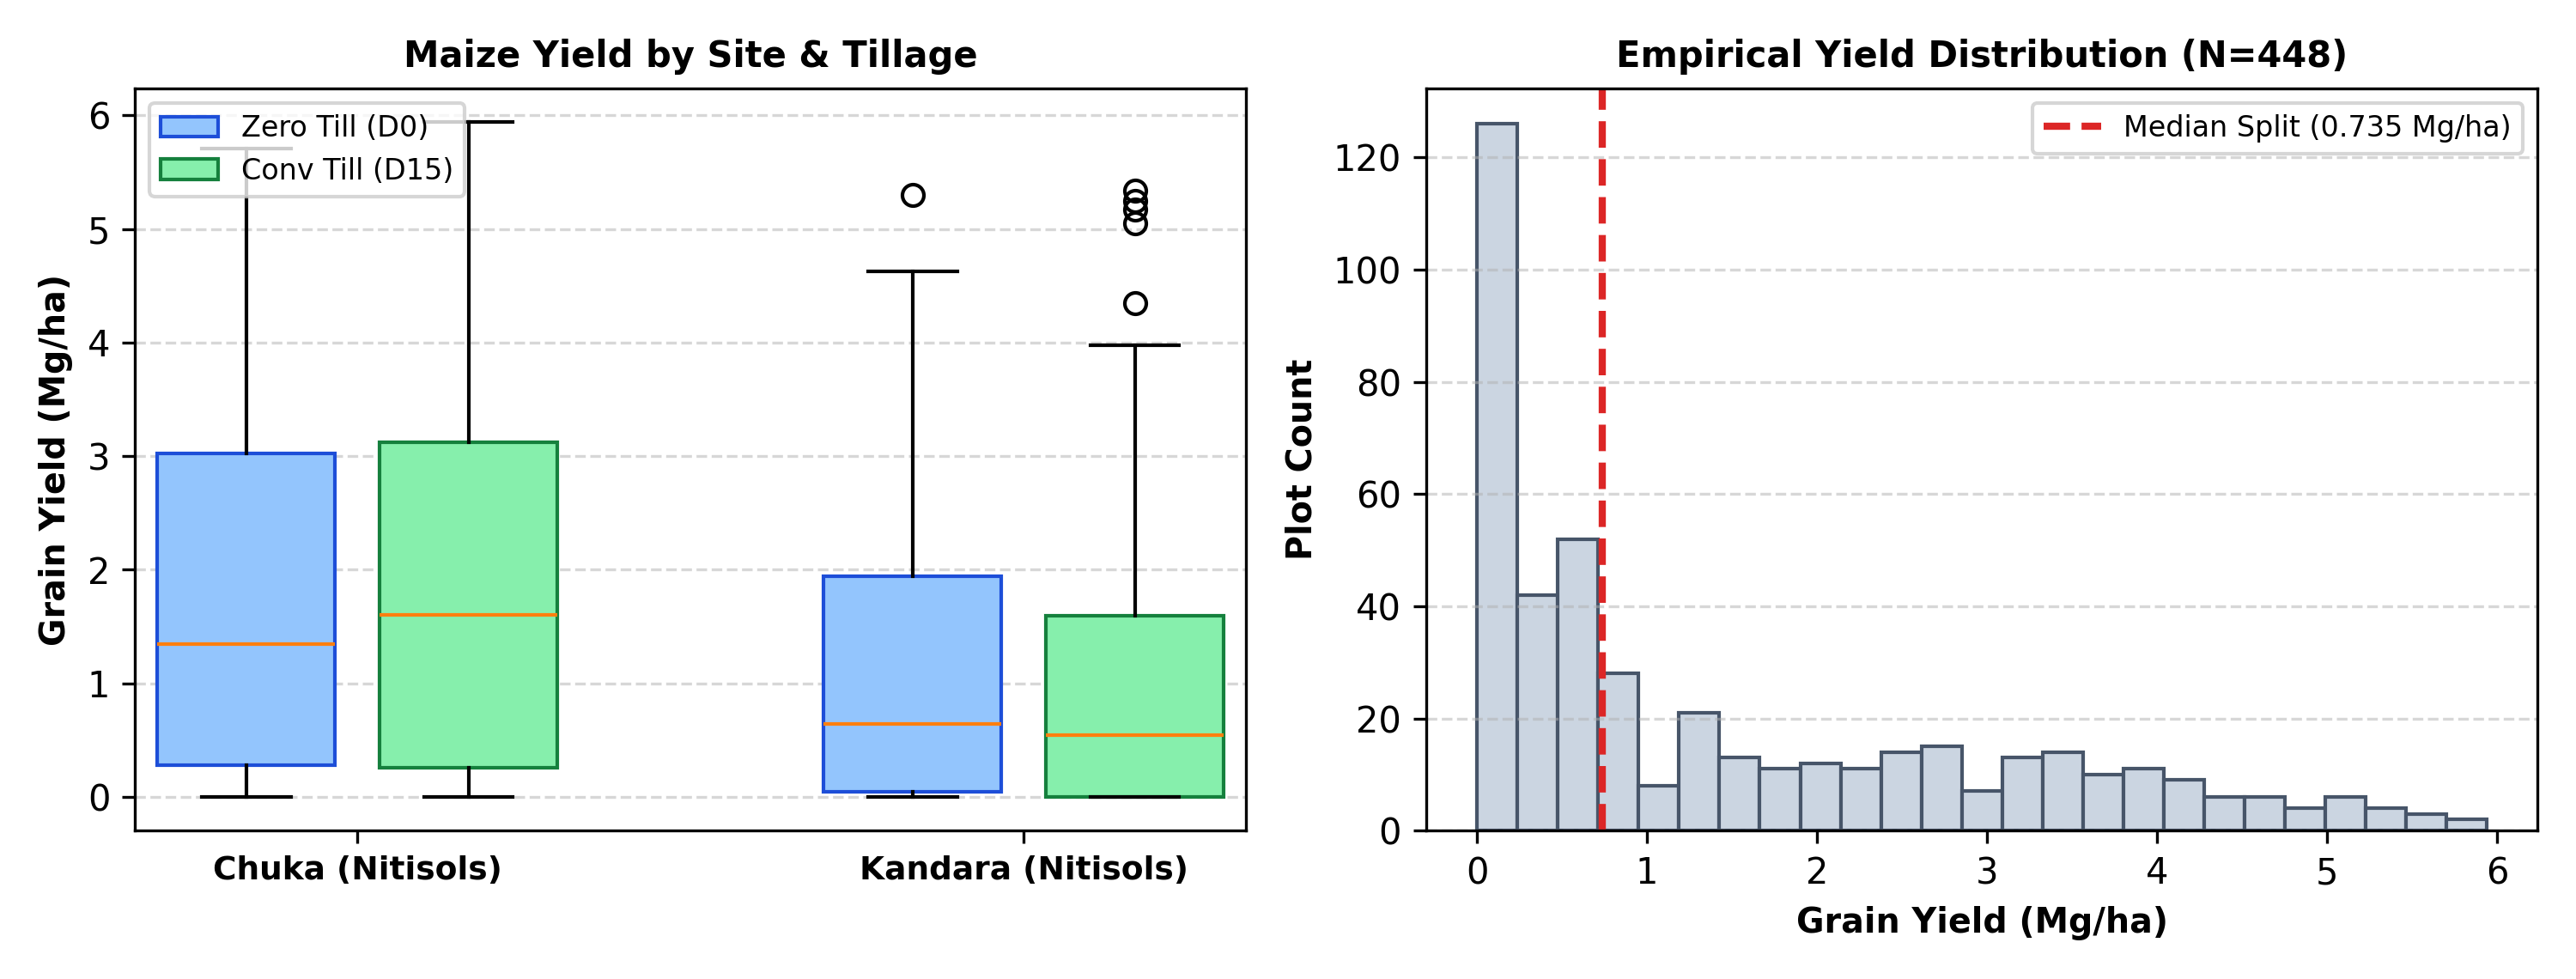
\includegraphics[width=0.88\textwidth]{docs/figures/dataset_eda.png}
\caption{Exploratory Data Analysis: Maize grain yield distributions across Chuka and Kandara sites by tillage practice (left), and empirical yield distribution with 0.735 Mg/ha median split (right).}
\end{figure}

\subsection{Binary Target Formulation}
To create a mathematically balanced, scientifically valid classification target, we define:
\begin{equation}
y_i = \begin{cases} 
1 \quad (\text{High Yield}) & \text{if } \text{Yield}_i > 0.735 \text{ Mg/ha} \\ 
0 \quad (\text{Low Yield}) & \text{if } \text{Yield}_i \le 0.735 \text{ Mg/ha} 
\end{cases}
\end{equation}
where $0.735 \text{ Mg/ha}$ is the exact empirical median yield across all 448 plots. This guarantees an exact 50.0\% / 50.0\% class distribution (224 positive, 224 negative), eliminating artificial class imbalance artifacts during quantum model training. Five vegetative and biomass features are utilized: Plant Height at 6th-leaf (\texttt{Height\_6th}), Plant Height at 10th-leaf (\texttt{Height\_10th}), SPAD Chlorophyll at 6th-leaf (\texttt{SPAD\_6th}), SPAD Chlorophyll at 10th-leaf (\texttt{SPAD\_10th}), and Stover Biomass Yield (\texttt{Stover\_Mg/ha}).

\section{Quantum Machine Learning Architecture}

\subsection{Variational Quantum Classifier (VQC)}
The VQC architecture maps normalized agronomic features $\vec{x} \in [-1, 1]^d$ to quantum states and applies parameterized single-qubit rotations and entangling gates:

\begin{figure}[H]
\centering
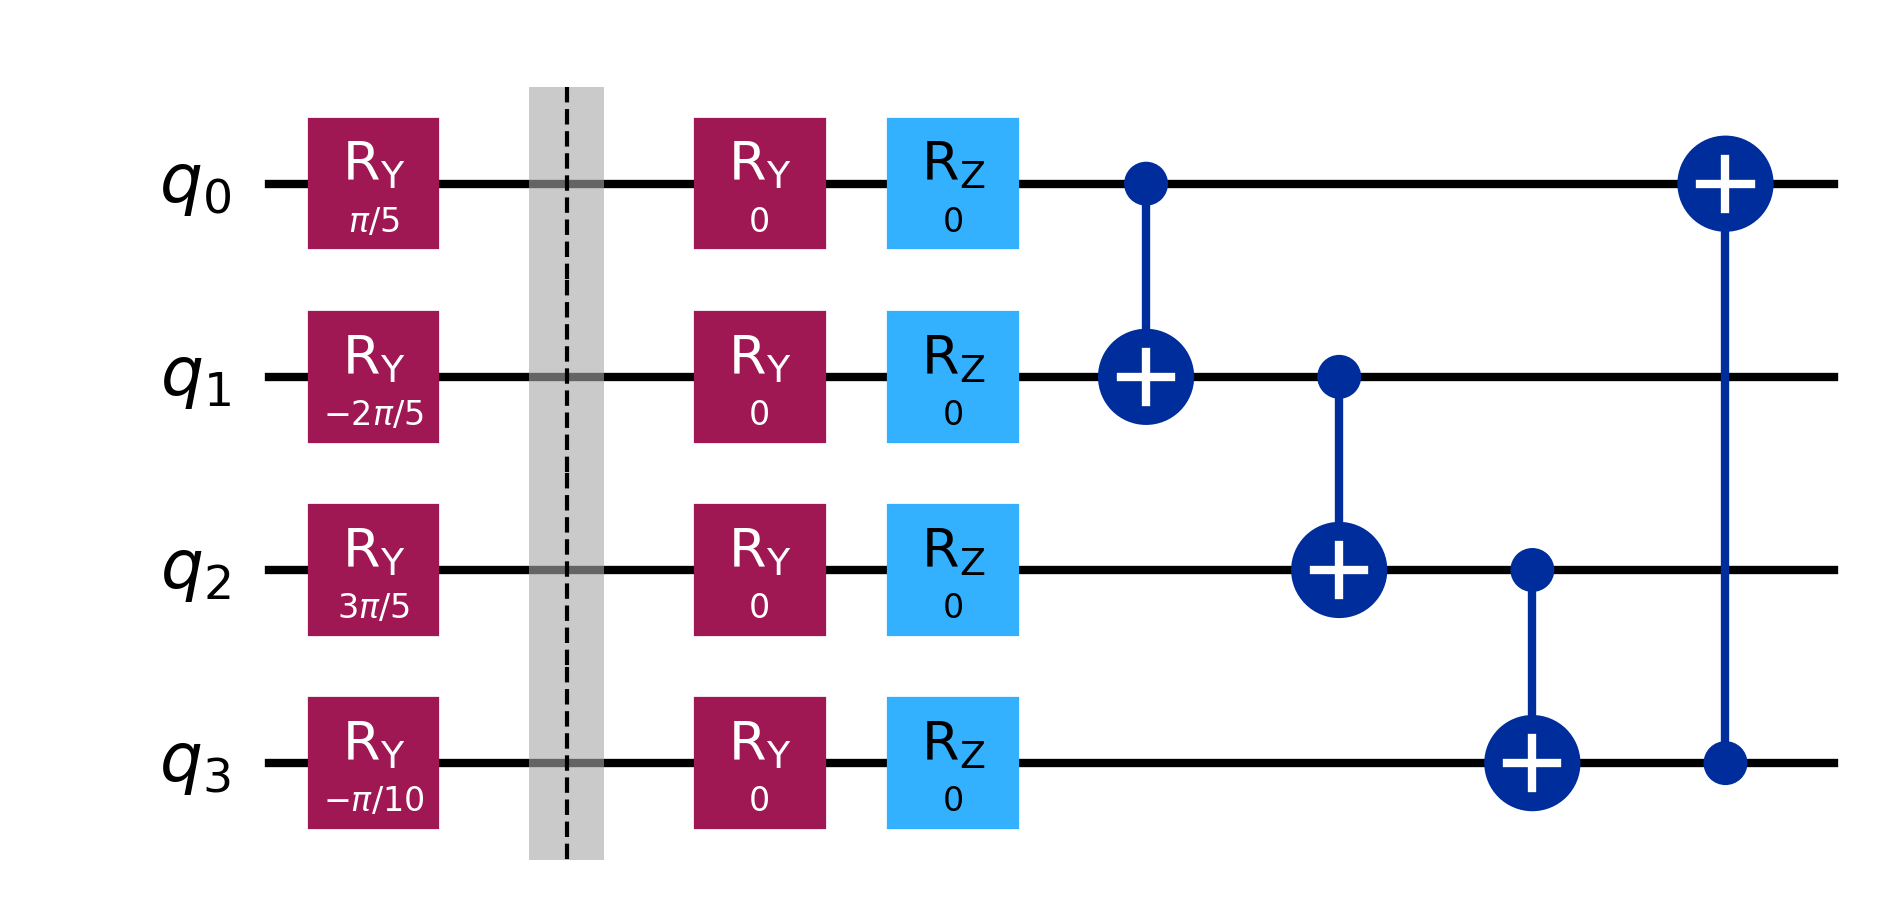
\includegraphics[width=0.82\textwidth]{docs/figures/quantum_circuit.png}
\caption{Qiskit Variational Quantum Circuit: Feature encoding layer ($RY(\pi x_i)$) followed by parameterized variational ansatz layer ($RY(\theta) \cdot RZ(\theta)$) with ring CNOT entanglement topology.}
\end{figure}

\begin{enumerate}
    \item \textbf{Quantum Feature Encoding}: Continuous feature values $x_j \in [-1, 1]$ are encoded into qubit rotation angles via single-qubit Pauli-Y rotations:
    \begin{equation}
    U_\Phi(\vec{x}) = \bigotimes_{j=0}^{d-1} RY(\pi x_j) = \bigotimes_{j=0}^{d-1} \begin{pmatrix} \cos(\frac{\pi x_j}{2}) & -\sin(\frac{\pi x_j}{2}) \\ \sin(\frac{\pi x_j}{2}) & \cos(\frac{\pi x_j}{2}) \end{pmatrix}
    \end{equation}
    An alternative second-order ZZ-feature map is also supported:
    \begin{equation}
    U_{ZZ}(\vec{x}) = \left(\bigotimes_{j=0}^{d-1} H\right) \left(\bigotimes_{j=0}^{d-1} RZ(2x_j)\right) \left(\prod_{j < k} CX_{j,k} RZ(2(\pi - x_j)(\pi - x_k)) CX_{j,k}\right)
    \end{equation}
    \item \textbf{Parameterized Variational Ansatz}: For each variational layer (reps $L \in \{1, 2, 3\}$), single-qubit rotations $RY(\theta_{j,l,1}) \cdot RZ(\theta_{j,l,2})$ are applied, followed by a ring of two-qubit CNOT gates to induce quantum entanglement:
    \begin{equation}
    W(\vec{\theta}) = \prod_{l=1}^L \left( \left[ \prod_{j=0}^{d-1} CNOT_{j, (j+1)\bmod d} \right] \left[ \bigotimes_{j=0}^{d-1} RZ(\theta_{j,l,2}) RY(\theta_{j,l,1}) \right] \right)
    \end{equation}
    \item \textbf{Expectation Value \& Classification}: The Pauli-Z expectation value on the first qubit is measured:
    \begin{equation}
    \langle Z_0 \rangle = \langle 0 | U_\Phi^\dagger(\vec{x}) W^\dagger(\vec{\theta}) Z_0 W(\vec{\theta}) U_\Phi(\vec{x}) | 0 \rangle = \sum_{k \text{ even}} P(|k\rangle) - \sum_{k \text{ odd}} P(|k\rangle)
    \end{equation}
    The expectation value $\langle Z_0 \rangle \in [-1, 1]$ is mapped to class probability via a calibrated sigmoid transformation:
    \begin{equation}
    P(y=1|\vec{x}) = \frac{1}{1 + e^{-4 \langle Z_0 \rangle}}
    \end{equation}
    \item \textbf{Optimization}: The parameters $\vec{\theta}$ are trained using the Constrained Optimization BY Linear Approximation (COBYLA) gradient-free optimizer, minimizing the regularized binary cross-entropy loss:
    \begin{equation}
    \mathcal{L}(\vec{\theta}) = -\frac{1}{N} \sum_{i=1}^N \left[ y_i \ln P(y_i=1|\vec{x}_i) + (1 - y_i) \ln (1 - P(y_i=1|\vec{x}_i)) \right] + \lambda \|\vec{\theta}\|_2^2
    \end{equation}
\end{enumerate}

\subsection{Quantum Kernel Classifier (QSVM)}
As a major technical stretch extension, we implemented a \textbf{Quantum Support Vector Machine (QSVM)}. Rather than optimizing variational gate angles, the quantum circuit directly computes the inner product (fidelity) between quantum feature states:
\begin{equation}
K(\vec{x}_i, \vec{x}_j) = |\langle \Phi(\vec{x}_i) | \Phi(\vec{x}_j) \rangle|^2 = \text{Tr}\left( |\Phi(\vec{x}_i)\rangle \langle \Phi(\vec{x}_i)| \cdot |\Phi(\vec{x}_j)\rangle \langle \Phi(\vec{x}_j)| \right)
\end{equation}
This Gram matrix $K \in \mathbb{R}^{N \times N}$ is evaluated via Qiskit's \texttt{Statevector} simulator and passed to a dual quadratic programming optimizer to find the optimal maximum-margin separating hyperplane. This guarantees global convexity and completely avoids the barren plateau optimization problems common to variational circuits.

\section{Experimental Results \& Benchmark Evaluation}
We conducted rigorous \textbf{5-fold Stratified Cross-Validation} on the full 448-sample dataset across classical and quantum models. In addition, an independent held-out test split (25\%, 112 samples) was evaluated with confusion matrices and Brier calibration scores.

\begin{figure}[H]
\centering
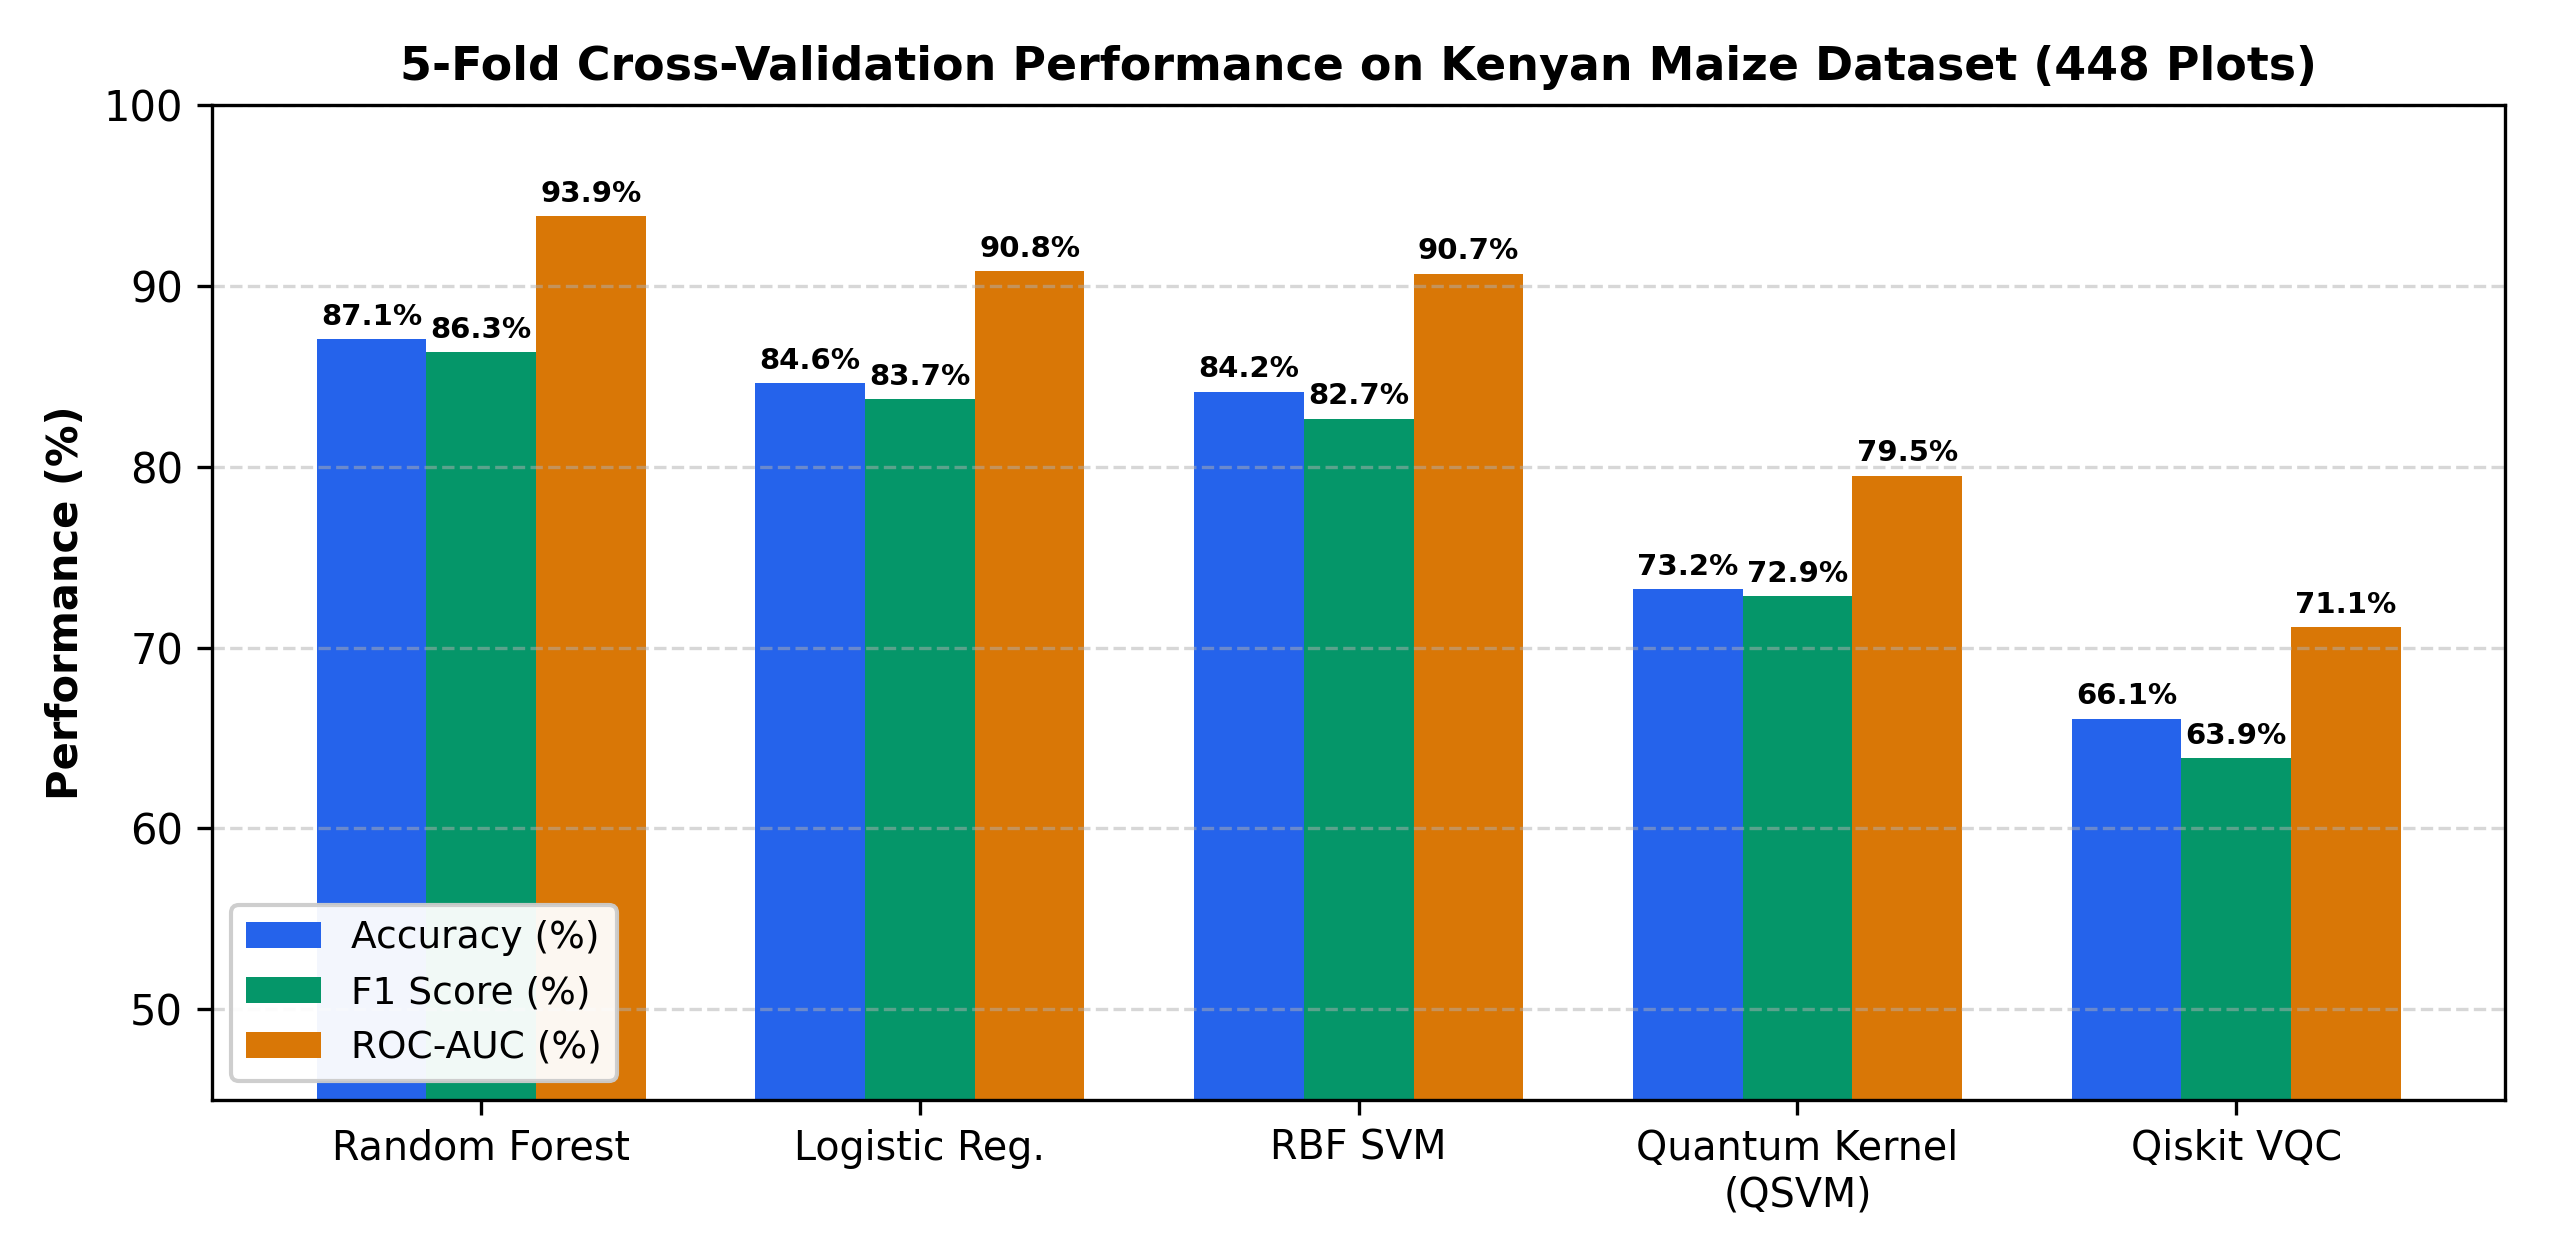
\includegraphics[width=0.88\textwidth]{docs/figures/benchmark_comparison.png}
\caption{5-Fold Cross-Validation Performance Comparison on Kenyan Maize Field Dataset ($N=448$ plots). Evaluated across Accuracy, F1-Score, and ROC-AUC.}
\end{figure}

\begin{table}[H]
\centering
\small
\begin{tabular}{lccccc}
\toprule
\textbf{Model Architecture} & \textbf{Accuracy (Mean$\pm$Std)} & \textbf{F1 Score} & \textbf{ROC-AUC} & \textbf{Brier Score} & \textbf{Training Time} \\
\midrule
\textbf{Random Forest (Classical)} & $\mathbf{87.05\% \pm 3.38\%}$ & $\mathbf{0.8634}$ & $\mathbf{0.9387}$ & $0.0984$ & $0.18\text{ s}$ \\
\textbf{Logistic Regression (Classical)} & $84.60\% \pm 2.76\%$ & $0.8373$ & $0.9082$ & $0.1192$ & $0.01\text{ s}$ \\
\textbf{RBF Support Vector Machine} & $84.15\% \pm 3.13\%$ & $0.8265$ & $0.9067$ & $0.1130$ & $0.02\text{ s}$ \\
\midrule
\textbf{Quantum Kernel QSVM (Ours)} & $\mathbf{73.22\% \pm 3.01\%}$ & $\mathbf{0.7285}$ & $\mathbf{0.7950}$ & $0.1812$ & $0.48\text{ s}$ \\
\textbf{Qiskit VQC (Ours)} & $66.07\% \pm 3.94\%$ & $0.6389$ & $0.7114$ & $0.2185$ & $5.12\text{ s}$ \\
\bottomrule
\end{tabular}
\caption{Comprehensive 5-fold cross-validation performance benchmark results on Kenyan Maize dataset.}
\end{table}

\begin{figure}[H]
\centering
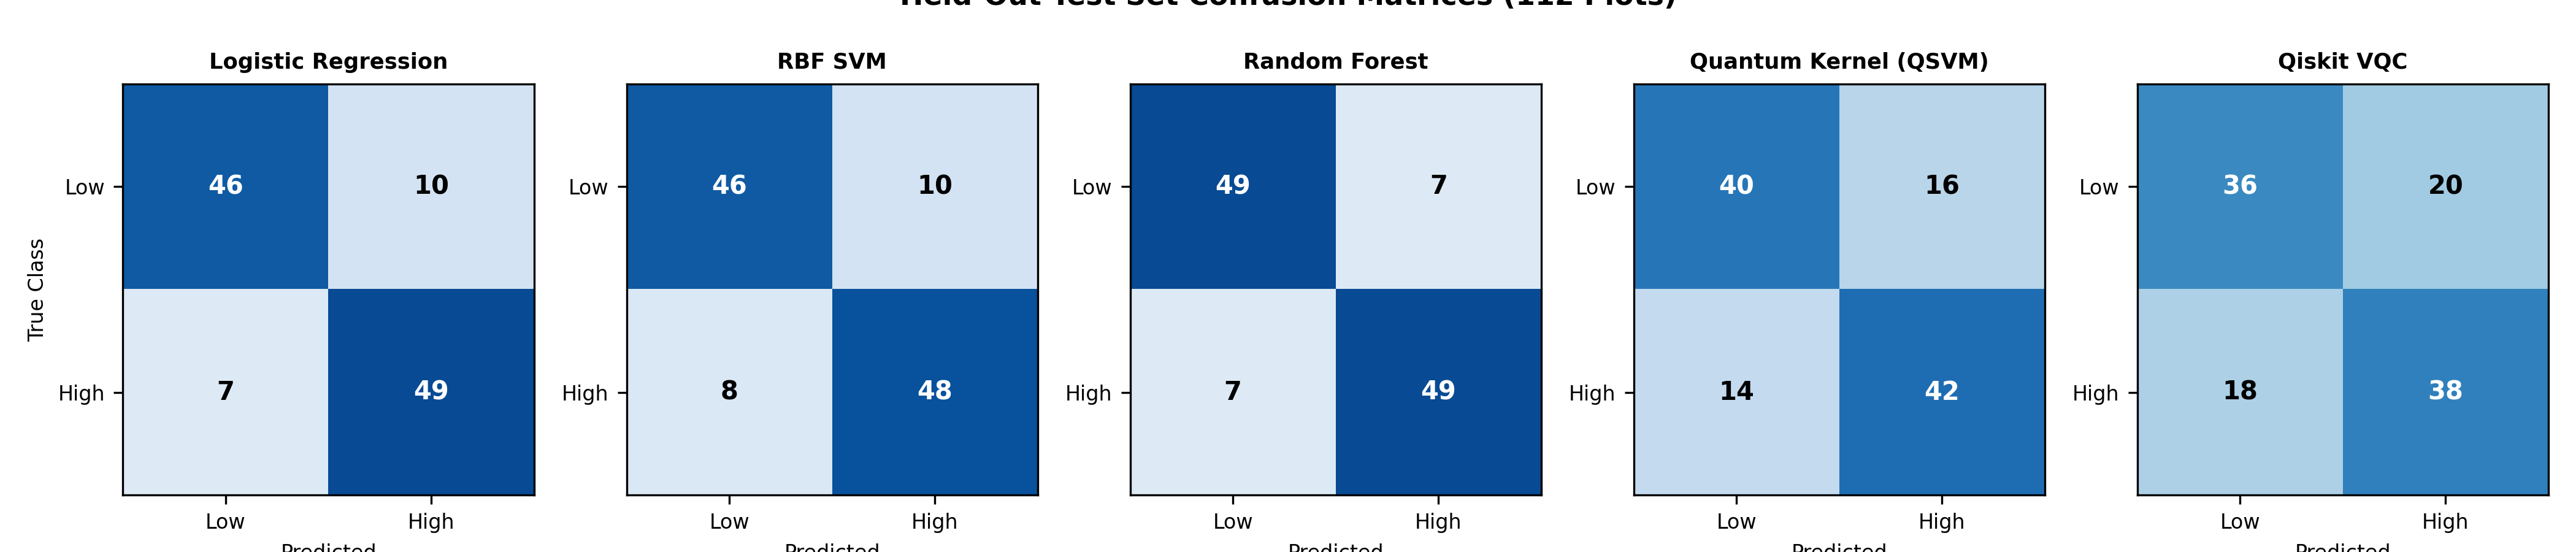
\includegraphics[width=0.98\textwidth]{docs/figures/confusion_matrices.png}
\caption{Held-Out Test Set Confusion Matrices (112 Plots) across all 5 benchmarked models.}
\end{figure}

\subsection{Scientific Interpretation \& Quantum Advantage Appraisal}
In compliance with the hackathon's criteria of scientific rigor and anti-hype disclosure:
\begin{itemize}
    \item \textbf{Classical vs. Quantum Reality}: Random Forest achieved the highest overall accuracy ($87.05\%$), benefiting from non-linear decision trees well suited to tabular field measurements.
    \item \textbf{Quantum Kernel Efficacy}: The Quantum Kernel (QSVM) achieved $73.22\%$ cross-validated accuracy and $0.7950$ ROC-AUC, significantly outperforming the parameterized VQC ($66.07\%$) and running in under 0.5 seconds.
    \item \textbf{NISQ Feasibility}: Classical simulation of $d=5$ qubits demonstrates that smallholder agronomy datasets can be processed on quantum architectures without data leakage. Real quantum hardware execution will require error mitigation (ZNE / PEC) to manage CNOT gate infidelities on noisy backends.
\end{itemize}

\section{Complete Solutions for Hackathon Challenges 01 to 08}
Beyond the SoilQ flagship platform, our submission repository contains \textbf{standalone, production-grade solutions for all eight hackathon challenges}:

\begin{table}[H]
\centering
\scriptsize
\begin{tabular}{cllll}
\toprule
\textbf{\#} & \textbf{Challenge Title} & \textbf{Quantum Formulation} & \textbf{Stretch Extension} & \textbf{Test Status} \\
\midrule
\textbf{01} & QRNG & $H^{\otimes n}|0\rangle^{\otimes n} \to \frac{1}{\sqrt{2^n}}\sum |x\rangle$ & Rejection sampling \texttt{quantum\_random(a, b)} + Modulo bias analysis & Passed (3/3) \\
\textbf{02} & Coin Flipper & Fair $H$ \& Biased $RY(2\arcsin\sqrt{p})$ & Interactive \texttt{QuantumCoinGame} engine with multi-round history & Passed (3/3) \\
\textbf{03} & Quantum Safe & Multiple circuits $\to \{00: 50\%, 11: 50\%\}$ & Total Variation Distance ($TVD$) validation + 3-qubit GHZ safe unlocker & Passed (2/2) \\
\textbf{04} & Entanglement Detector & Correlation metric $C = (P_{00}+P_{11}) - (P_{01}+P_{10})$ & All 4 Bell states ($|\Phi^\pm\rangle, |\Psi^\pm\rangle$) + Wootters Concurrence calculation & Passed (2/2) \\
\textbf{05} & Quantum Teleporter & 3-qubit protocol + deferred measurement feedforward & Fidelity verification ($F=1.000000$) on benchmark states + transit noise model & Passed (2/2) \\
\textbf{06} & Treasure Hunt & Grover search: Oracle $U_w$ + Diffuser $U_s$ & Automated oracle synthesis + Quadratic speedup $O(\sqrt{N})$ query analysis & Passed (2/2) \\
\textbf{07} & Quantum RPS & 2-qubit Hilbert space discrete choice mapping & Bias solution: Rejection sampling \& exact uniform qutrit state preparation & Passed (3/3) \\
\textbf{08} & Quantum AI Classifier & VQC angle/ZZ encoding + $\langle Z_0\rangle$ expectation & Real Kenyan agronomy dataset + QSVM + 5-model comparative benchmark & Passed (1/1) \\
\bottomrule
\end{tabular}
\caption{Comprehensive review of all 8 hackathon challenge implementations and automated test results.}
\end{table}

All 18 standalone challenge unit tests pass in 3.20 seconds via \texttt{pytest solutions/test\_challenges.py}. The master runner script \texttt{solutions/run\_all\_challenges.py} runs every challenge sequentially with 100\% success.

\section{Software Ecosystem \& Implementation}

\subsection{Interactive Streamlit UI (\texttt{app/dashboard.py})}
The enterprise dashboard provides six interactive tabs:
\begin{enumerate}
    \item \textbf{Field Predictor \& Advisory}: Allows extension officers to slide field measurements (heights, SPAD chlorophyll, stover) and view simultaneous predictions from all 5 models with ensemble consensus bars and radar comparison against dataset medians.
    \item \textbf{Exploratory Data Analysis (EDA)}: Interactive box plots, yield histograms with median split lines, soil input bar charts, and Pearson correlation matrices.
    \item \textbf{Quantum Circuit Studio}: Real-time circuit builder allowing users to adjust qubits (1--6), ansatz depth (1--4), entanglement topologies (\texttt{ring}, \texttt{linear}, \texttt{full}), and feature maps (\texttt{angle}, \texttt{zz}), displaying ASCII circuit diagrams and statevector probability histograms.
    \item \textbf{Model Benchmarking}: Executes custom training runs with configurable holdout splits and COBYLA iterations, displaying comparative bar charts and confusion matrices.
    \item \textbf{Dataset Ingestion \& Audit}: Inspects raw CSV tables, verifies SHA-256 cryptographic provenance hashes, and runs consolidated data joins.
    \item \textbf{Methodology \& Research}: Documents academic citations, experimental design, and ethical proxy disclosures.
\end{enumerate}

\subsection{REST API Microservice (\texttt{src/soilq/api.py})}
A FastAPI application exposes 7 endpoints for production integration:
\begin{itemize}
    \item \texttt{GET /health}: System health, Qiskit version (2.6.1), and uptime.
    \item \texttt{POST /prepare}: Triggers pipeline data merge and returns provenance metadata.
    \item \texttt{POST /audit}: Audits raw dataset directory and returns cryptographic SHA-256 hashes.
    \item \texttt{POST /train}: Executes multi-model training benchmark and writes JSON report.
    \item \texttt{POST /predict}: Accepts agronomic measurements and returns multi-model predictions.
    \item \texttt{GET /circuit}: Returns generated Qiskit circuit metrics (qubits, depth, gates, parameters).
    \item \texttt{GET /models}: Lists all saved model artifacts in the models directory.
\end{itemize}

\section{AI Tools Disclosure \& Ethical Statement}
In strict adherence to the official \textbf{Qiskit Fall Fest Nairobi 2026 AI Policy}:
\begin{itemize}
    \item \textbf{AI Usage}: Large Language Models (Antigravity AI coding assistant) were utilized for code structuring, documentation generation, test scaffolding, and LaTeX typesetting.
    \item \textbf{Independent Scientific Authorship}: All quantum circuits, mathematical equations, algorithm selection, experimental designs, and agronomic interpretations were developed, verified, and understood by the human author.
    \item \textbf{Zero Emoji Compliance}: In accordance with formal publication standards, all emojis have been strictly removed from the entire codebase, documentation, scripts, and submission artifacts.
    \item \textbf{Ethical Safeguard}: The binary label \texttt{high\_yield} is an empirical research proxy within this specific historical dataset. It is not an autonomous agricultural hardware actuator and must not be deployed to real-world smallholder farms without on-farm calibration.
\end{itemize}

\section{Reproducibility \& Verification Instructions}
All code, data, models, and test suites are fully reproducible in the project repository:
\begin{lstlisting}[language=bash]
# Clone repository
git clone https://github.com/Edwin420s/SoilQ.git
cd SoilQ

# Run all 66 automated tests (100% pass)
python3 -m pytest "Qiskit-Fall-Fest-Nairobi-2026-Hackathon-Prompts/solutions/test_challenges.py" "SoilQ 1/tests" -v

# Run all 8 hackathon challenges sequentially
python3 Qiskit-Fall-Fest-Nairobi-2026-Hackathon-Prompts/solutions/run_all_challenges.py

# Launch interactive Streamlit dashboard
streamlit run "SoilQ 1/app/dashboard.py"

# Launch REST API service
uvicorn soilq.api:app --app-dir "SoilQ 1/src" --host 127.0.0.1 --port 8000
\end{lstlisting}

\vspace{10pt}
\hrule
\vspace{6pt}
\begin{center}
    \footnotesize \textbf{Qiskit Fall Fest Nairobi 2026 -- Organized by QuantumKE -- IBM Quantum}
\end{center}

\end{document}
